\documentclass{bmstu}

\usepackage{mathtools}

\usepackage{physics}
\usepackage{pdfpages}
\usepackage{tabularx}
\usepackage{longtable}
\usepackage{xfrac}
\usepackage{amssymb}
\usepackage{dsfont}
\usepackage{upgreek}
\usepackage{color, colortbl}
\usepackage{listings}
\usepackage{ amssymb }
\usepackage{tikz}
\usetikzlibrary{decorations.markings}
\usetikzlibrary{calc} 
\usepackage{ wasysym }

\begin{document}
	\section*{06/12}
	\begin{center}
		\textbf{Сохранение непрерывности вдоль границ между элементами}
	\end{center}

\begin{center}
	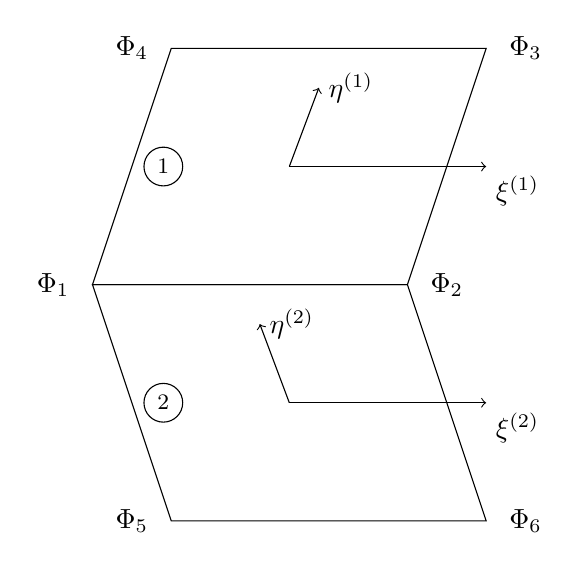
\begin{tikzpicture}
		\draw (0,0) -- (4,0) -- (5,3) -- (1,3) -- cycle;
		\draw(0.9,1.5) circle(7pt);
		\node at (0.9,1.5) {\footnotesize 1};
		\draw[->] (2.5,1.5) -- (5,1.5) node[below right] {$\xi^{(1)}$};
		\draw[->] (2.5,1.5) -- (2.875,2.5) node[right] {$\eta^{(1)}$};
		\node at (-0.5,0) {$\Phi_1$};
		\node at (4.5,0) {$\Phi_2$};
		\node at (5.5,3) {$\Phi_3$};
		\node at (0.5,3) {$\Phi_4$};
		\draw (0,0) -- (4,0) -- (5,-3) -- (1,-3) -- cycle;
		\draw(0.9,-1.5) circle(7pt);
		\node at (0.9,-1.5) {\footnotesize 2};
		\draw[->] (2.5,-1.5) -- (5,-1.5) node[below right] {$\xi^{(2)}$};
		\draw[->] (2.5,-1.5) -- (2.125,-0.5) node[right] {$\eta^{(2)}$};
		\node at (0.5,-3) {$\Phi_5$};
		\node at (5.5,-3) {$\Phi_6$};
	\end{tikzpicture}
\end{center}

\[
\begin{cases}
	\varphi^{(1)}=N_1^{(1)}\Phi_1+N_2^{(1)}\Phi_2+N_3^{(1)}\Phi_3+N_4^{(1)}\Phi_4 \\
	\varphi^{(2)}=N_1^{(2)}\Phi_5+N_2^{(2)}\Phi_6+N_3^{(2)}\Phi_2+N_4^{(2)}\Phi_1
\end{cases}
\]
\[
	\begin{cases}
	N_1=\frac{1}{4}(1-\xi)(1-\eta) \\
	N_2=\frac{1}{4}(1+\xi)(1-\eta) \\
	N_3=\frac{1}{4}(1+\xi)(1+\eta) \\
	N_4=\frac{1}{4}(1-\xi)(1+\eta)
	\end{cases} 
\]
\[
	\eta^{(1)}=-1, \eta^{(2)}=1  \Rightarrow  \begin{cases}
	\varphi^{(1)}=\frac{1}{2}(1-\xi^{(1)})\Phi_1 + \frac{1}{2}(1+\xi^{(1)})\Phi_2 \\
	\varphi^{(2)}=\frac{1}{2}(1+\xi^{(2)})\Phi_2 + \frac{1}{2}(1-\xi^{(2)})\Phi_1
	\end{cases}
\]
\[
	\xi^{(1)}=\xi^{(2)} \Rightarrow \varphi^{(1)}=\varphi^{(2)}
\]

\begin{center}
	\textbf{Квадратичные и кубические четырехугольные КЭ из Серендипова семейства}
\end{center}
\[
\begin{cases}
\varphi_2=\alpha_1+\alpha_2x+\alpha_3y+\alpha_4xy+\alpha_5x^2y+\alpha_6xy^2+\alpha_7x^2+\alpha_8y^2 \\
\varphi_3= \alpha_1+\alpha_2x+\alpha_3y+\alpha_4xy+\alpha_5x^2y+\alpha_6xy^2+\alpha_7x^2+\alpha_8y^2 + \\
\qquad +\alpha_9x^3+\alpha_{10}y^3+\alpha_{11}x^3y+\alpha_{12}xy^3
\end{cases}
\]
\[
\Rightarrow
\begin{cases}
	N^{(2)}=(\alpha_1+\alpha_2\xi+\alpha_3\eta+\alpha_4\xi\eta)(a_1+a_2\xi+a_3\eta) \\
	N^{(3)}=(\alpha_1+\alpha_2\xi+\alpha_3\eta+\alpha_4\xi\eta)(a_1+a_2\xi+a_3\eta+a_4\xi^2+a_5\eta^2)
\end{cases}
\]

Для квадратичного элемента:

\begin{center}
	\begin{tikzpicture}
		\draw(0,0) -- (4,0) -- (4,3) -- (0,3) -- cycle;
		\draw[->] (0,1.5) -- (5, 1.5) node[below right] {$\xi$};
		\draw[->] (2,0) -- (2,4) node[right] {$\eta$};
		\fill (0,0) circle(1.5pt);
		\fill (2,0) circle(1.5pt);
		\fill (4,0) circle(1.5pt);
		\fill (4,1.5) circle(1.5pt);
		\fill (0,1.5) circle(1.5pt);
		\fill (4,3) circle(1.5pt);
		\fill (2,3) circle(1.5pt);
		\fill (0,3) circle(1.5pt);
		\fill (2,1.5) circle(1.5pt);
		\node at (0,-0.5) {\footnotesize 1};
		\node at (2,-0.5) {\footnotesize 2};
		\node at (4,-0.5) {\footnotesize 3};
		\node at (4.25,1.75) {\footnotesize 4};
		\node at (4.25,3.25) {\footnotesize 5};
		\node at (1.75,3.25) {\footnotesize 6};
		\node at (-0.25,3.25) {\footnotesize 7};
		\node at (-0.25,1.75) {\footnotesize 8};
		\node at (2.25,1.75) {\footnotesize 0};
	\end{tikzpicture}
\end{center}

Вычислим функцию формы для элемента 1:
\[
	N_1=(1-\eta)(1-\xi)(a_1+a_2\xi+a_3\eta) 
\]
\[ \begin{cases}
	N_1(\xi=0, \eta=1)=0 \\
	N_1(\xi=-1, \eta=0) =0 \\
	N_1(\xi=-1, \eta=1) = 1 \end{cases} \Rightarrow \begin{cases} N_1=2(a_1-a_3)=0 \\ N_1=2(a_1-a_2)=0 \\ N_1 = 4(a_1-a_2-a_3)=1  \end{cases}
\]
\[
\Rightarrow a_1=a_2=a_3=-\frac{1}{4} 
\]
\[
	\Rightarrow N_1=-\frac{1}{4}(1-\eta)(1-\xi)(1+\xi+\eta) 
\]

Вычислим функцию формы для элемента 2:
\[
N_2=(\alpha_1+\alpha_2\xi+\alpha_3\eta+\alpha_4\xi\eta)(a_1+a_2\xi+a_3\eta)=(1+\xi)(1-\xi)(1-\eta)\cdot a \Rightarrow
\]
\[
	\Rightarrow 
	N_2(\xi=0, \eta=-1)=2a=1\Rightarrow a=\frac{1}{2} \Rightarrow N_2=\frac{1}{2}(1-\xi^2)(1-\eta)
\]

Для кубического элемента:
\begin{center}
	\begin{tikzpicture}
		\draw(0,0) -- (4,0) -- (4,3) -- (0,3) -- cycle;
		\draw[->] (2,1.5) -- (5, 1.5) node[below right] {$\xi$};
		\draw[->] (2,1.5) -- (2,4) node[right] {$\eta$};
		\fill (0,0) circle(1.5pt);
		\fill (1.33,0) circle(1.5pt);
		\fill (2.66,0) circle(1.5pt);
		\fill (4,0) circle(1.5pt);
		\fill (4,1) circle(1.5pt);
		\fill (4,2) circle(1.5pt);
		\fill (0,1) circle(1.5pt);
		\fill (0,2) circle(1.5pt);
		\fill (4,3) circle(1.5pt);
		\fill (1.33,3) circle(1.5pt);
		\fill (2.66,3) circle(1.5pt);
		\fill (0,3) circle(1.5pt);
		\fill (2,1.5) circle(1.5pt);
		
		\node at (0,-0.5) {\footnotesize 1};
		\node at (1.33,-0.5) {\footnotesize 2};
		\node at (2.66,-0.5) {\footnotesize 3};
		\node at (4,-0.5) {\footnotesize 4};
		\node at (4.25,1) {\footnotesize 5};
		\node at (4.25,2) {\footnotesize 6};
		\node at (4.25,3.25) {\footnotesize 7};
		\node at (2.66,3.25) {\footnotesize 8};
		\node at (1.33,3.25) {\footnotesize 9};
		\node at (-0.25,3.25) {\footnotesize 10};
		\node at (-0.25,2) {\footnotesize 11};
		\node at (-0.25,1) {\footnotesize 12};
		\node at (2.25,1.75) {\footnotesize 0};
	\end{tikzpicture}
\end{center}
\[
N_1=(1-\xi)(1-\eta)(a_1+a_2\xi+a_3\eta+a_4\xi^2+a_5\eta^2)
\]
\[
\begin{cases}
	N_1(-\frac{1}{3},-1)=0  \\
	N_1(\frac{1}{3},-1)=0 \\
	N_1(-1,\frac{1}{3})=0 \\
	N_1(-1, -\frac{1}{3})=0 \\
	N_1(-1,-1)=1
\end{cases}
\]

\begin{center}
	\textbf{Вычисление производных}
\end{center}
\[
\begin{bmatrix}
	\frac{\partial N_{\beta}}{\partial \xi} \\
	\frac{\partial N_{\beta}}{\partial \eta}
\end{bmatrix} = \begin{bmatrix}
\frac{\partial x}{\partial \xi} & \frac{\partial x}{\partial \eta} \\
\frac{\partial y}{\partial \xi} & \frac{\partial y}{\partial \eta}
\end{bmatrix} \begin{bmatrix}
\frac{\partial N_{\beta}}{\partial x} \\
\frac{\partial N_{\beta}}{\partial y}
\end{bmatrix} = 
J \cdot \begin{bmatrix}
	\frac{\partial N_{\beta}}{\partial x} \\
	\frac{\partial N_{\beta}}{\partial y}
	\end{bmatrix}
\Rightarrow \begin{bmatrix}
\frac{\partial N_{\beta}}{\partial x} \\
\frac{\partial N_{\beta}}{\partial y}
\end{bmatrix}=J^{-1} \begin{bmatrix}
\frac{\partial N_{\beta}}{\partial \xi} \\
\frac{\partial N_{\beta}}{\partial \eta}
\end{bmatrix}
\]

Допустим, $\varphi_2=N_1\Phi_1+\dots+N_8\Phi_8$

Форма элемента прямолинейного четырехугольника:
\begin{center}
	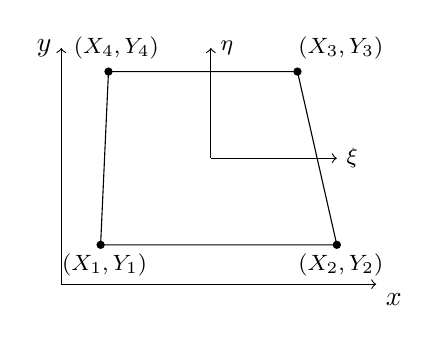
\begin{tikzpicture}
		\draw[->] (0,0) -- (4,0) node[below right] {$x$};
		\draw[->] (0,0) -- (0,3) node[left] {$y$};
		\draw (0.5,0.5) -- (3.5,0.5) -- (3,2.7) -- (0.6,2.7) -- cycle;
		\fill (0.5,0.5) circle (1.5pt);
		\fill (3.5,0.5) circle (1.5pt);
		\fill (3,2.7) circle (1.5pt);
		\fill (0.6,2.7) circle (1.5pt);
		\draw[->] (1.9,1.6) -- (3.5, 1.6) node[right] {\footnotesize $\xi$};
		\draw[->] (1.9,1.6) -- (1.9, 3) node[right] {\footnotesize $\eta$};
		\node at (0.55,0.25) {\footnotesize $(X_1,Y_1)$};
		\node at (3.55,0.25) {\footnotesize $(X_2,Y_2)$};
		\node at (3.55,3) {\footnotesize $(X_3,Y_3)$};
		\node at (0.7,3) {\footnotesize $(X_4,Y_4)$};
	\end{tikzpicture}
\end{center}
\[
\begin{cases}
	x=R_1X_1+R_2X_2+R_3X_3+R_4X_4 \\
	y=R_1Y_1+R_2Y_2+R_3Y_3+R_4Y_4
\end{cases}  \text{ -- субпараметрический КЭ}
\]

где $R_i$ - линейные интерполяции

\[
\begin{cases}
	R_1=\frac{1}{4}(1-\xi)(1-\eta) \\
	R_2=\frac{1}{4}(1+\xi)(1-\eta) \\
	R_3=\frac{1}{4}(1+\xi)(1+\eta) \\
	R_4=\frac{1}{4}(1-\xi)(1+\eta)
\end{cases}
\]

\newpage
Изопараметрический КЭ:
\begin{center}
	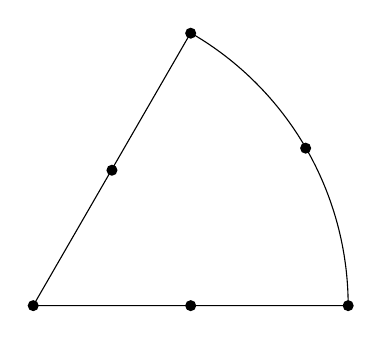
\begin{tikzpicture}[scale=2]
		\draw (0,0) -- (2,0) arc[start angle=0, end angle=60, radius=2] -- cycle;
		\fill (0,0) circle (1pt);
		\fill (1,0) circle (1pt);
		\fill (2,0) circle (1pt);
		\fill (1.73,1) circle (1pt);
		\fill (1,1.73) circle (1pt);
		\fill (0.5,0.86) circle (1pt);
	\end{tikzpicture}
\end{center}

\[
\begin{cases}
	x=N_1X_1+\dots+N_8X_8 \\
	y=N_1Y_1+\dots+N_8Y_8
\end{cases}
\]

Так как все стороны линейные, интегралы можно свести к виду:
\[
\int\limits_VB^TDB\ dV=t\int\limits_{-1}^1\int\limits_{-1}^1 B^TDB |J|\ d\eta d\xi
\]
\[
Z=\int\limits_{-1}^1\int\limits_{-1}^1 f(\xi, \eta) \ d\eta d\xi = \sum\limits_{i=1}^{n}\sum\limits_{j=1}^{n}H_iH_j f(\xi_i, \eta_j)
\]
\[
\int\limits_{-1}^1\int\limits_{-1}^1 f(\xi, \eta) \ d\eta =\sum\limits_{j=1}^{n} H_j f (\xi, \eta_j) = g(\xi)
\]
\[
\int\limits_{-1}^1 g(\xi)\ d\xi = \sum\limits_{i=1}^{n} H_i g(\xi_i)
\]

\begin{center}
	\textbf{Лагранжево семейство}
\end{center}

\begin{center}
	\begin{tikzpicture}
		\draw (0,0) rectangle (4,1.5);
		\fill (0,0.75) circle (1.5pt);
		\fill (2,0.75) circle (1.5pt);
		\fill (4,0.75) circle (1.5pt);
		\draw (0,-2) rectangle (4,-0.5);
		\fill (1.33,-1.25) circle (1.5pt);
		\fill (2.66,-1.25) circle (1.5pt);


		\draw(6,-2) -- (10,-2) -- (10,1) -- (6,1) -- cycle;
		\fill (6,-2) circle(1.5pt);
		\fill (8,-2) circle(1.5pt);
		\fill (10,-2) circle(1.5pt);
		\fill (10,-0.5) circle(1.5pt);
		\fill (6,-0.5) circle(1.5pt);
		\fill (10,1) circle(1.5pt);
		\fill (8,1) circle(1.5pt);
		\fill (6,1) circle(1.5pt);
		\fill (8,-0.5) circle(1.5pt);
		\node at (6,-2.5) {\footnotesize 1};
		\node at (8,-2.5) {\footnotesize 2};
		\node at (10,-2.5) {\footnotesize 3};
		\node at (10.25,-0.25) {\footnotesize 4};
		\node at (10.25,1.25) {\footnotesize 5};
		\node at (7.75,1.25) {\footnotesize 6};
		\node at (5.75,1.25) {\footnotesize 7};
		\node at (5.75,-0.25) {\footnotesize 8};
		\node at (8.25,-0.25) {\footnotesize 9};
	\end{tikzpicture}
\end{center}

Функция формы:
\[
N_{ij}=L_i^n(\xi)L_j^m(\eta)
\]

$L_i^n(\xi)L_j^m(\eta)$ - многочлены Лагранжа, $n,m$ - количество разбиений по $\xi, \eta$

\[
L_i^n(\xi)=\frac{(\xi-\xi_1)(\xi-\xi_2)\dots(\xi-\xi_n)}{(\xi_i-\xi_1)(\xi_i-\xi_2)\dots(\xi_i-\xi_n)}
\]
\[
N_{ij}=L_i^2(\xi)L_j^2(\eta),\ i \neq 1,2
\]
\[
L_i^2(\xi)=\frac{(\xi-\xi_1)(\xi-\xi_2)}{(\xi_i-\xi_1)(\xi_i-\xi_2)}
\]
\\
\begin{center}
	\begin{tikzpicture}
		\draw (0,0) -- (4,0);
		\fill (0,0) circle(1.5pt);
		\fill (2,0) circle(1.5pt);
		\fill (4,0) circle(1.5pt);
		\node at (0,-0.5) {$i = -1$};
		\node at (2,-0.5) {$\xi_1 = 0$};
		\node at (4,-0.5) {$\xi_2 = 1$};

		\draw (0,-2) -- (4,-2);
		\fill (0,-2) circle(1.5pt);
		\fill (2,-2) circle(1.5pt);
		\fill (4,-2) circle(1.5pt);
		\node at (0,-2.5) {$\xi_1$};
		\node at (2,-2.5) {$i$};
		\node at (4,-2.5) {$\xi_2$};
	\end{tikzpicture}
\end{center}

\[
N_{11}=\frac{\xi\cdot(\xi-1)}{-1\cdot(-2)}\cdot \frac{\eta\cdot(\eta-1)}{-1\cdot(-2)}=\frac{1}{4}\cdot\xi\cdot\eta (\xi-1)(\eta-1)
\]
\[
N_{12}=\frac{\xi\cdot(\xi-1)}{2}\cdot \frac{(\eta+1)(\eta-1)}{1\cdot(-1)}
\]
\begin{center}
	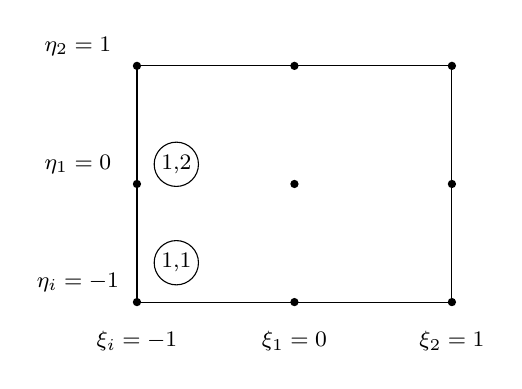
\begin{tikzpicture}
		\draw(0,0) -- (4,0) -- (4,3) -- (0,3) -- cycle;
		\fill (0,0) circle(1.5pt);
		\fill (2,0) circle(1.5pt);
		\fill (4,0) circle(1.5pt);
		\fill (4,1.5) circle(1.5pt);
		\fill (0,1.5) circle(1.5pt);
		\fill (4,3) circle(1.5pt);
		\fill (2,3) circle(1.5pt);
		\fill (0,3) circle(1.5pt);
		\fill (2,1.5) circle(1.5pt);
		\node at (0,-0.5) {\footnotesize $\xi_i=-1$};
		\node at (2,-0.5) {\footnotesize $\xi_1=0$};
		\node at (4,-0.5) {\footnotesize $\xi_2=1$};

		\node at (-0.75,3.25) {\footnotesize $\eta_2=1$};
		\node at (-0.75,1.75) {\footnotesize $\eta_1=0$};
		\node at (-0.75,0.25) {\footnotesize $\eta_i=-1$};

		\draw(0.5,0.5) circle(8pt);
		\node at (0.5,0.5) {\footnotesize 1,1};

		\draw(0.5,1.75) circle(8pt);
		\node at (0.5,1.75) {\footnotesize 1,2};
	\end{tikzpicture}
\end{center}

\end{document}